

\begin{problem} (10 points)
  Consider the relation structure shown below:

  \bigskip

  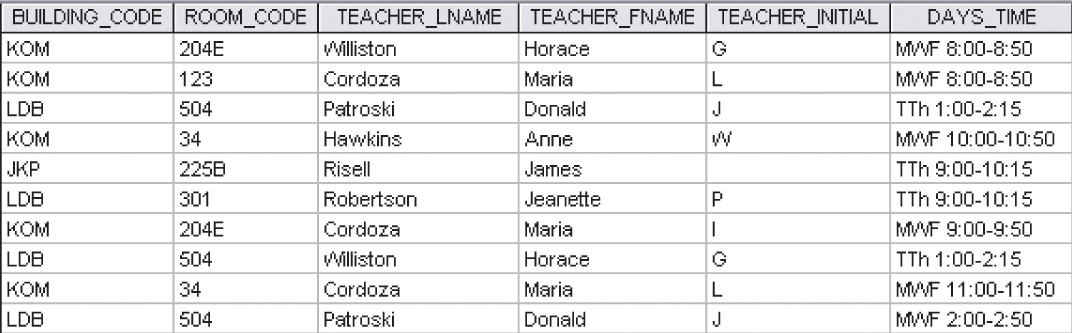
\includegraphics[scale=0.8]{01.png}

  \begin{enumalph}
    \item Identify and discuss the serious data redundancy problems.
    \begin{Answer}
      The main data redundancy in the \cw{TEACHER_LNAME}
      and \cw{TEACHER_FNAME} fields:
      \begin{enumalph}
        \item ``Cordoza Maria'' occurs $3$ times.
        \item ``Willstone Horace'' occurs $2$ times.
        \item ``Patroski Donald'' occurs $2$ times.
      \end{enumalph}
	
      \bigskip
      This redundancy requires that any update to a row (tuple) containing
      any of those three be reflected across every other rows containing the same.
      Otherwise, the data will be inconsistent.
      Indeed, we see ``Cordoza Maria'' having two initials: ``L'' and ``I''.
      It is likely that one initial is outdated, but the change
      was not broadcast to all rows containing the ``Cordoza Maria'' combination
      for \cw{TEACHER_LNAME} and \cw{TEACHER_FNAME}.

      The relation structure should be normalized so that
      each update needs to happen only at a single place.
    \end{Answer}
    \item  If this relation is the only one describing the teaching schedule,
    what problems might arise if the KOM building was condemned
    and every row referring to that building was deleted?
    \begin{Answer}

      Deleting all rows (tuples) referring to the KOM building
      would result int he loss of all data for
      Horace Williston, Cordoza Maria, and Hawkins Anne.
      Their existence in the system, including details such as their
      \cw{TEACHER_INITIAL} and \cw{DAYS_TIME} would be lost
      despite not being dependent on the \cw{BUILDING_CODE}.
      A better data model would extract those attributes into separate tables
      to have atomic data.
    \end{Answer}
  \end{enumalph}

\end{problem}
